\begin{block}{Project Features}
    \begin{itemize}
        \item Obtain and evaluate source code from compressed file or
            tools such as Git, Subversion, and Bazaar.
        \item Code processing scheduling.
        \item Use of multiple metrics configurations for multiple
            projects.
        \item Visualization of results per file via plot graphics.
        \item Public results that are accessible by the community.
        \item Extensible architecture to include new metric collectors.
            Currently, the following collectors are available:
            \begin{itemize}
                \item Analizo
                \item metric\_fu
                \item Radon
                \item CodeClimatePHPMD
            \end{itemize}
    \end{itemize}
\end{block}

\begin{block}{Metric evaluation results.}
    \begin{figure}
        \begin{center}
            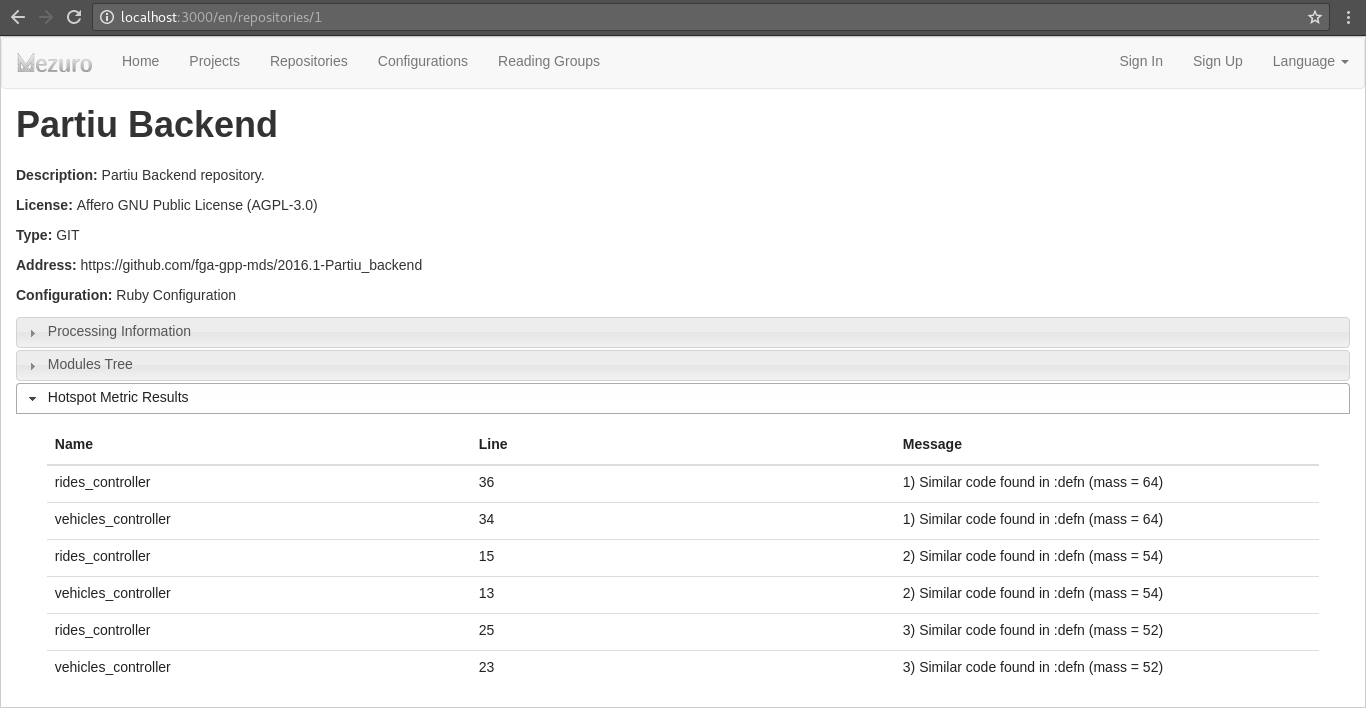
\includegraphics[width=\textwidth]{figures/MetricProcessing.png}
                \label{fig:feature1}
        \end{center}
    \end{figure}
\end{block}

\begin{block}{Metric Configurations Features}
    \begin{itemize}
        \item Metric configurations features are responsible for allowing
            definitions and spread of metrics configurations, being
            one of Mezuro stand out factors among the others platforms.
            \begin{itemize}
                \item Metrics creation.
                \item Metrics configuration cloning, giving users a quick start
                    to rate their projects, and the option to use already well
                    established metrics configuration.
                \item Statistics about most popular configurations in the
                    community.
                \item Creation of ``reading groups'' to be used in textual
                    interpretation of metrics results.
                \item Configuration of qualitative ranges associated with
                    value of metrics.
                \item Combination of native metrics to create composed and more
                    complex analysis.
            \end{itemize}
    \end{itemize}
\end{block}

\begin{block}{Reading groups}
    \begin{figure}
        \begin{center}
            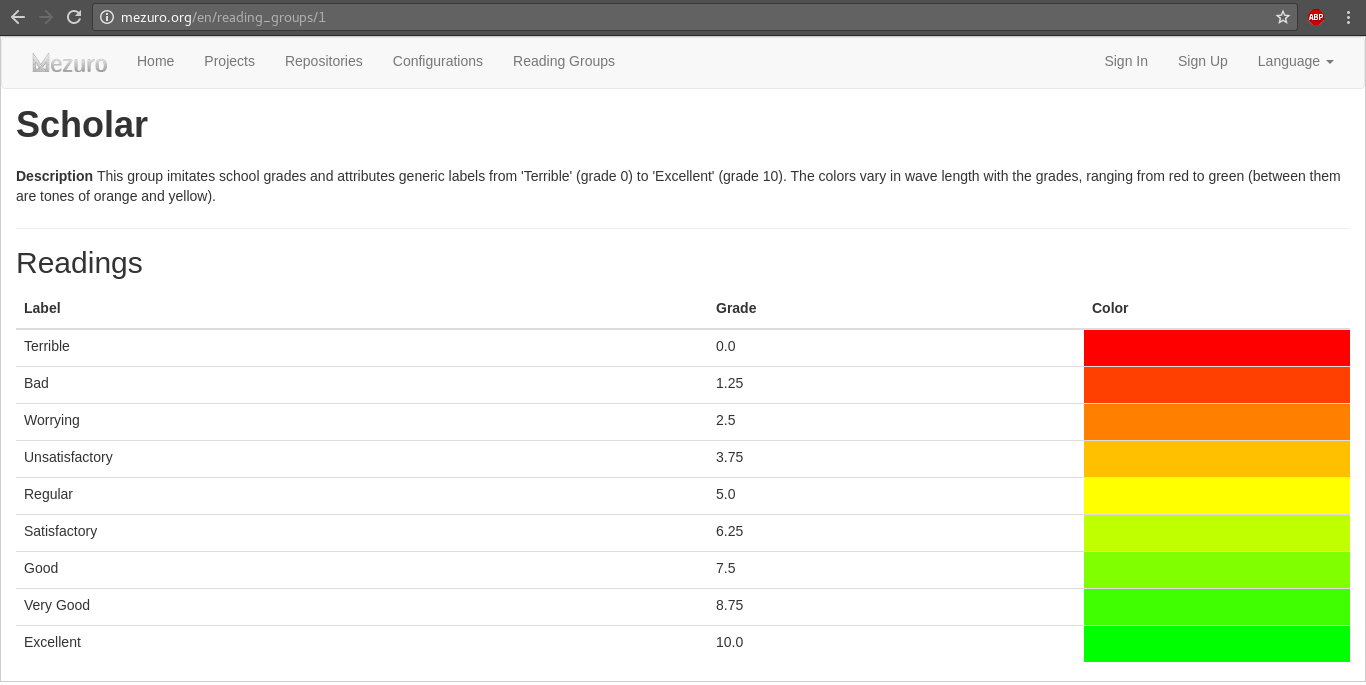
\includegraphics[width=\textwidth]{figures/ReadingGroup.png}
            \label{fig:feature1}
        \end{center}
    \end{figure}
\end{block}

\begin{block}{Next Steps}
    \begin{itemize}
        \item Frontend enhancement.
        \item Improvement of processing elapsed time.
        \item Transfer for Gitlab CI (from Travis).
        \item Auto-detection of repository language.
    \end{itemize}
\end{block}
